%------------------------------------------------------------------------------------------------
	\section{Architecture}
%------------------------------------------------------------------------------------------------
The API has been designed to enable a strong separation between the {\em controller} of an experiment and the testbed(s) ({\em testbed service(s)}) being controlled, to the extent that the controller software can be either co-located with the testbed services, or located on the testbed user's personal computer.

In the following, \ssecref{arch-overview} introduces the general idea of the architecture and \ssecref{arch-examples} describes a number of concrete realisations of this API.

%------------------------------------------------------------------------------------------------
	\subsection{Overview}
	\label{ssec:arch-overview}
%------------------------------------------------------------------------------------------------
The API is divided vertically into two `roles':
\begin{itemize}
	\item the testbed service role, and 
	\item the controller role. 
\end{itemize}

The testbed service role implements all of the functions which are directed at a testbed; while the controller role implements the functions which are directed at a controller (often these are responses to functions previously directed at a testbed by that controller). This division is shown in \figref{architecture1}, which also provides the key for the remaining figures in this section. Note that a controller may become inaccessible during an experiment -- for example due to loss of Internet connectivity -- and return at a later point; in such cases a reconnecting controller should be informed of any events occurring in its absence.

	\begin{figure}[htb]
		\centering
		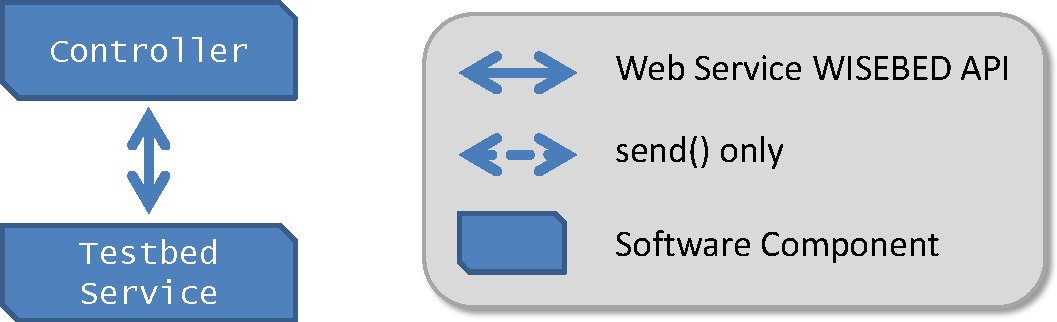
\includegraphics[width=0.75\columnwidth]{images/architecture1}
		\caption{}
		\label{fig:architecture1}
	\end{figure}

Implementations of the WISEBED APIs are designed to be hierarchically composable, such that one instance can drive -- and receive feedback from -- another instance (cf. \figref{architecture2}). This also means that an entity controlling an experiment -- driving a WSN API -- does not need to be aware of a possible hierarchy of API instances below that `root' instance. This permits arbitrary federations and virtualisations of testbeds that are controllable by the same controller.

	\begin{figure}[htb]
		\centering
		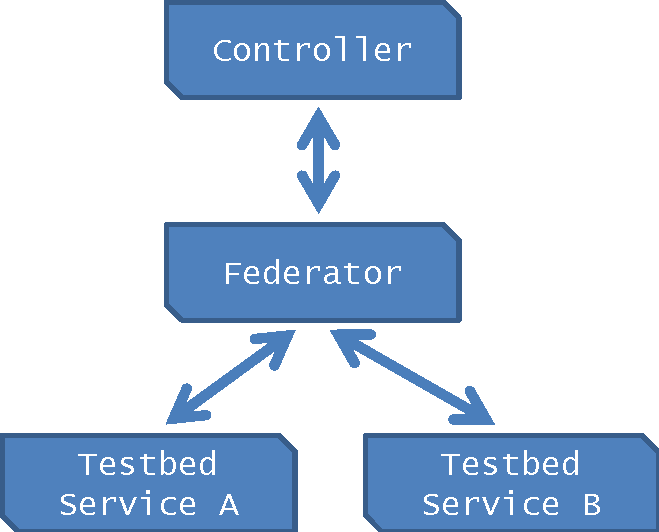
\includegraphics[width=0.5\columnwidth]{images/architecture2}
		\caption{}
		\label{fig:architecture2}
	\end{figure}

The proposed API also operates to support the communication required for virtual links within a federated testbed architecture. As illustrated in \figref{architecture3}, this communication is supported directly between the two testbed services involved in a virtual link. A second method of virtual link communication is also supported such that the sending of a message can travel through a third `testbed service proxy' which contains some custom filter or virtual link behaviour (cf. \figref{architecture4}). These two virtual link communication methods are supported using the same API, since a virtual link end-point is described by using the WSN API end-point (i.e. testbed service) address and the WSN node to which the link is targeted.

\begin{figure}[htbp]
	\begin{center}
		\mbox
		{
			\subfigure[Between two testbeds] { 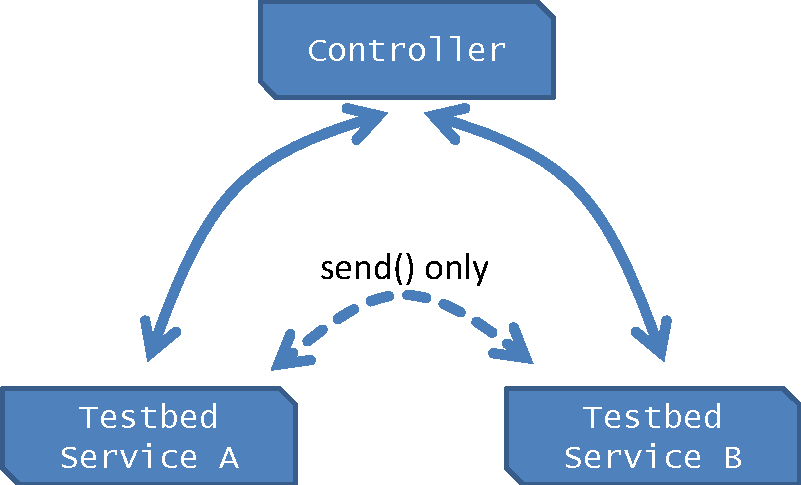
\includegraphics[width=.45\columnwidth]{images/architecture3} \label{fig:architecture3} } 
			\quad
			\subfigure[Using a `testbed service proxy']	{ 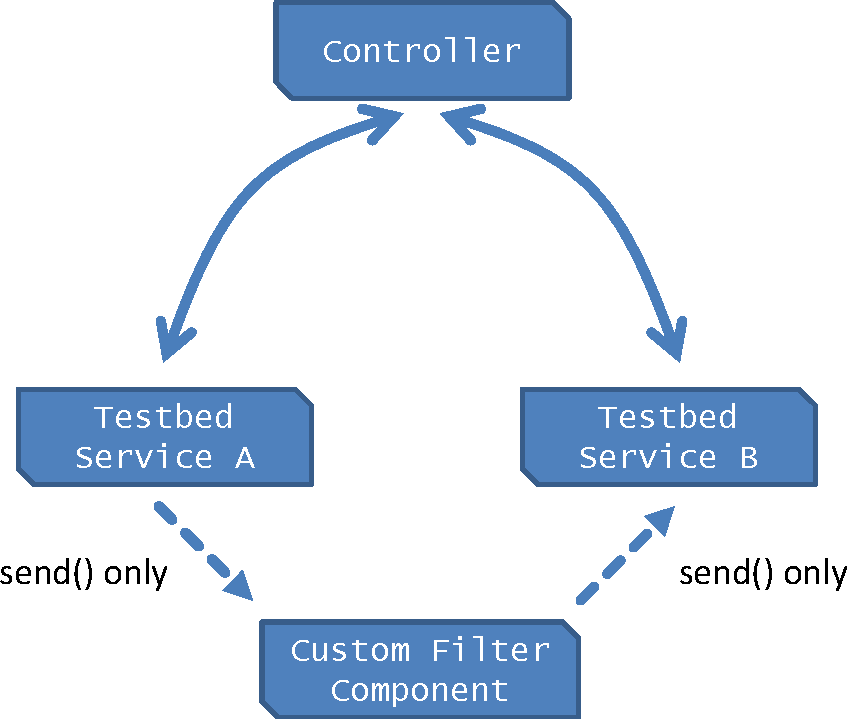
\includegraphics[width=.35\columnwidth]{images/architecture4} \label{fig:architecture4} }
		}
		\caption{Virtual Link Communication}
		\label{fig:architecture-vlinks}
	\end{center}
\end{figure}	

The general flow of control for a user of the WISEBED federation is therefore as follows: 
\begin{itemize}
	
	\item They are first authorized to use the federation and authenticated by an external security system (e.g. via some web-based sign-up procedure). 
	
	\item They then use an external reservation system (again perhaps through a website) which provides that user with access to selected testbed resources at some point in the future and returns to them a `reservation ID'. As mentioned previously the details of both of these systems are beyond the scope of this document. 
	
	\item When a user's reserved time arrives they -- or a system working on their behalf -- can use their reservation ID to acquire the reference(s) to the testbed service instance(s) at the revelant site(s). These instances will be destroyed automatically when their reserved time expires. 

\end{itemize}

%------------------------------------------------------------------------------------------------
	\subsection{Concrete Realisations}
	\label{ssec:arch-examples}
%------------------------------------------------------------------------------------------------
Having presented the abstract architecture proposed by this API revision we now describe a number of concrete realisations of this API.

The first case is the simplest where a single testbed is being used (cf. \figref{architecture5}). Here there is no architectural change from WSN API 1.0. The second case (\figref{architecture6}) allows multiple testbeds to be {\em federated} into a single virtual network using a special aggregating testbed service called a Federator. A controller using such a federated virtual testbed simply sees a single network accessed via a single WSN API instance, abstracting the details of virtualisation.
% \question{Which network node is responsible for spawning the federating instance? In case of unfederated testbeds it is pretty clear that the testbed service acting as experiment controlling gateway to the sensor nodes should spawn an instance for a new experiment. For federated a clear definition of responsibilities is missing.}\\
% \proposal{I can think of two situations: \begin{enumerate}
% 	\item There's some federating service running on some physical machine exposing a federated testbed that can be reserved for experiments as a whole. In this case it's easy to define that this physical machine is responsible to spawn an instance.
% 	\item WSN testbed are federated dynamically for each experiment based on the selection of nodes an experimenter wants to use. The nodes can totally be spread over different testbeds. In this case I don't have a good idea yet how to define responsibilities.
% \end{enumerate}}

The strong separation of Controller and Testbed Service roles additionally permit the WISEBED APIs to be used to control (using a simple controller) a pure simulation on a local computer. \figref{architecture8} shows an example where a simulation running in Shawn is controlled by the controller as, e.g., the one shown in \figref{architecture5} and \figref{architecture6}. Finally, we can employ the same concept as above to use a simple controller for a purely local/private testbed which is physically connected to the user's computer as shown in \figref{architecture9}.
% \question{Who (e.g. which physical machine) is responsible to start a simulation, e.g. a shawn instance upon experiment start?}\\
% \proposal{IMO it doesn't make sense to run the simulation in the controllers machine as a controller instance will typically not be available 24/7 or even not for the duration of an experiment. Therefore it must be placed on some kind of "server", providing maximum uptime and computation resources.}

\begin{figure}[htbp]
	\begin{center}
		\mbox
		{
			\subfigure[Single Testbed] { 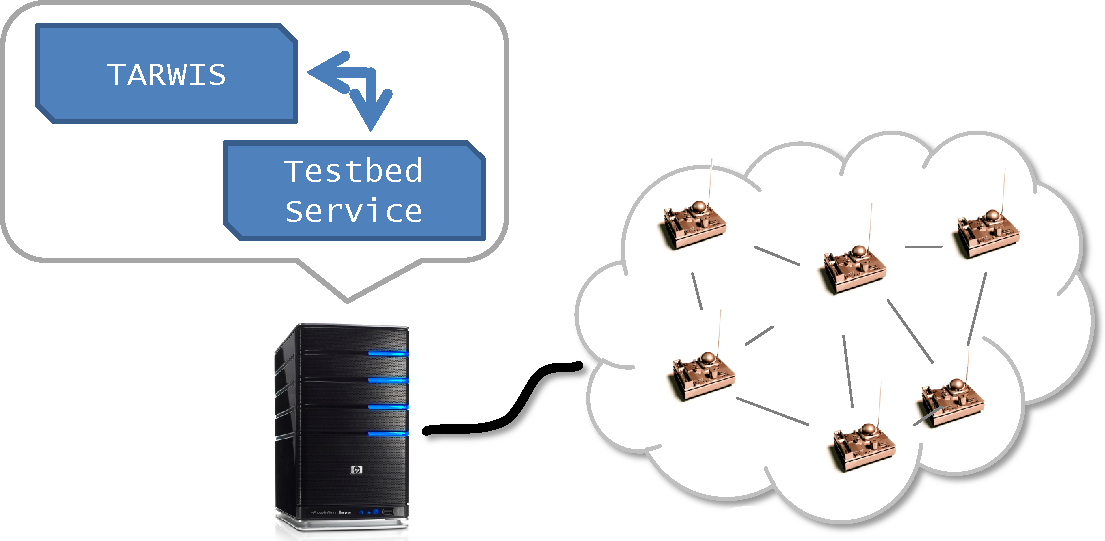
\includegraphics[width=.5\columnwidth]{images/architecture5} \label{fig:architecture5} } 
			\quad
			\subfigure[Federation of multiple testbeds]	{ 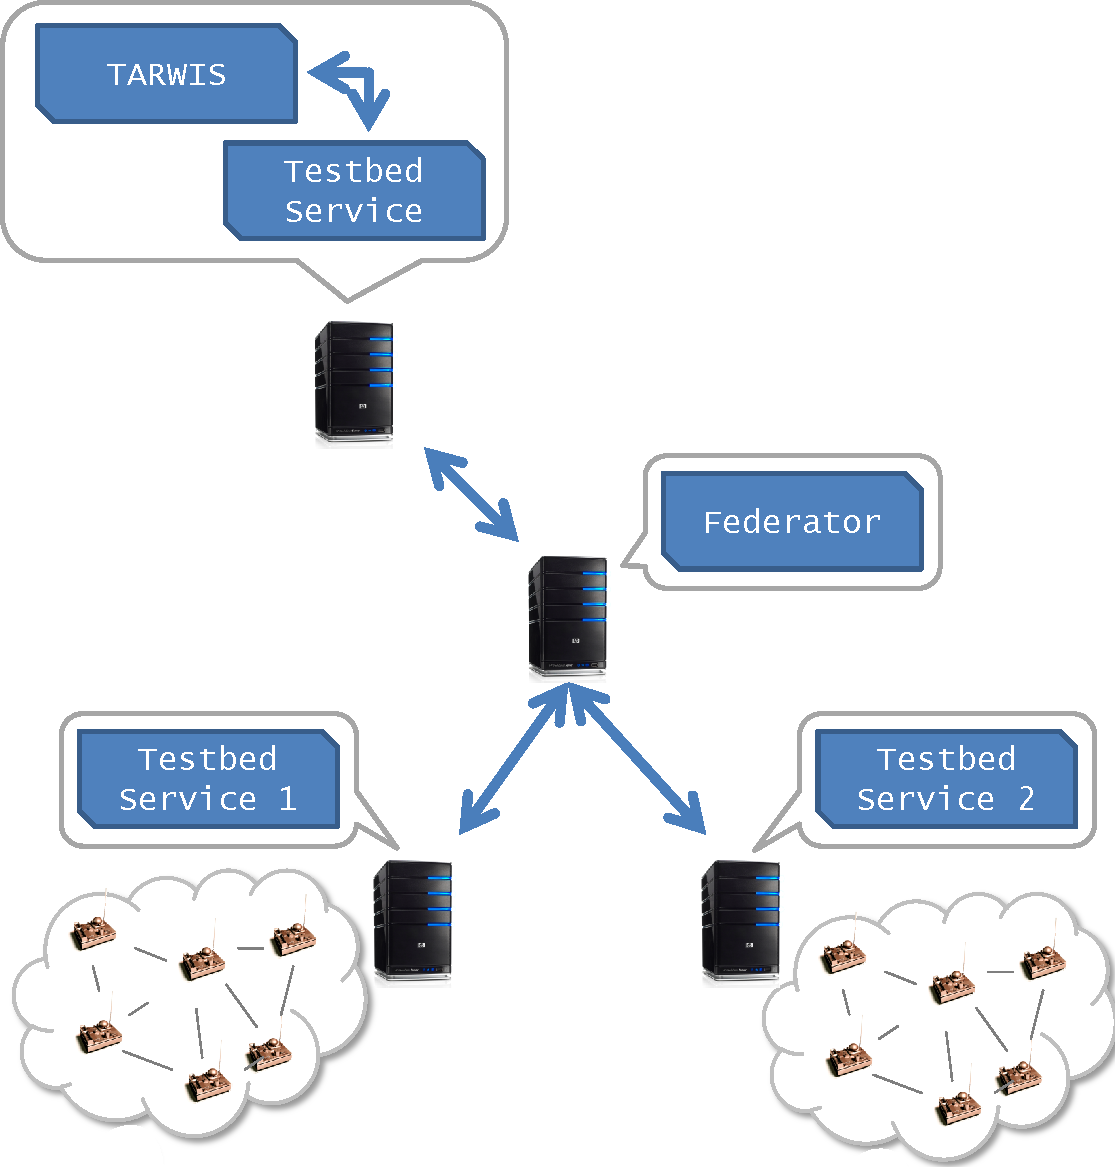
\includegraphics[width=.3\columnwidth]{images/architecture6} \label{fig:architecture6} }
		}
		\caption{Single vs. Federated Testbed usage}
		\label{fig:architecture5and6}
	\end{center}
\end{figure}	

\begin{figure}[htbp]
	\begin{center}
		\mbox
		{
			\subfigure[Controlling a simulated testbed] { 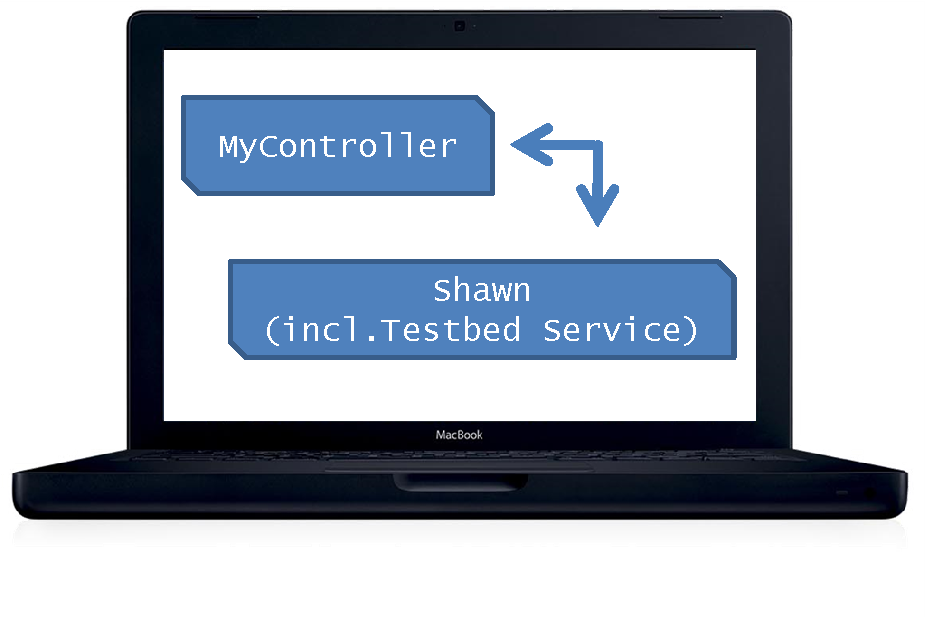
\includegraphics[width=.35\columnwidth]{images/architecture8} \label{fig:architecture8} } 
			\quad
			\subfigure[Controlling a `private' testbed attached]	{ 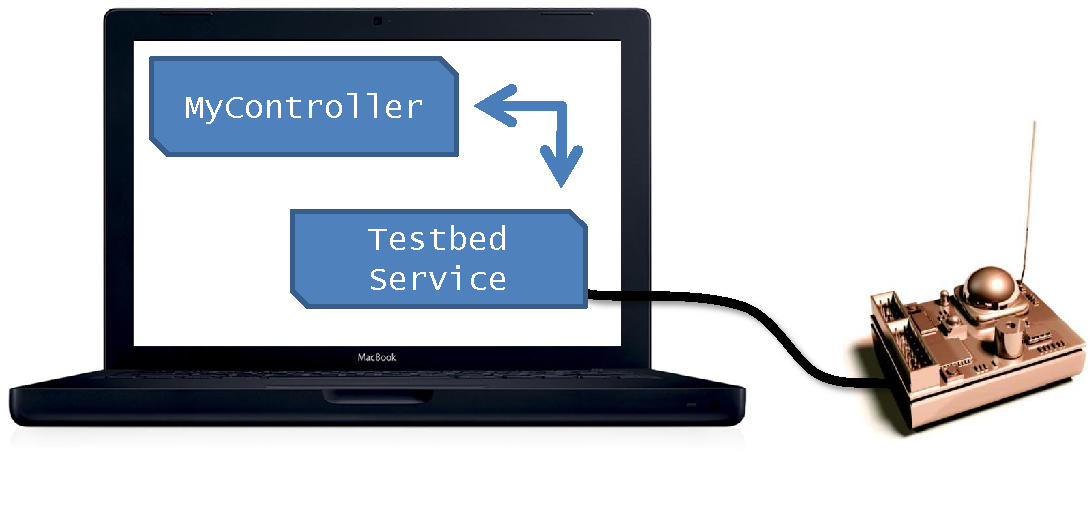
\includegraphics[width=.5\columnwidth]{images/architecture9} \label{fig:architecture9} }
		}
		\caption{Different setups of `private' testbeds}
		\label{fig:architecture8and9}
	\end{center}
\end{figure}	
